\documentclass[10pt,aspectratio=169]{beamer}

\usetheme{AICL}

\usepackage{amsmath, amssymb}
\usepackage{booktabs}
\usepackage{graphicx}
\usepackage{tikz}
\usetikzlibrary{arrows.meta, positioning, shapes.geometric}

\graphicspath{{../figures/}}

\title{Pilot Assignment in Cell-Free Massive MIMO}
\subtitle{System Model, Pilot Contamination, and Adaptive Assignment}
\author{Myoungjin Oh \and Jeonghoo Maeng}
\date{June 2026}

\newcommand{\taup}{\tau_{\mathrm{p}}}
\newcommand{\tauc}{\tau_{\mathrm{c}}}
\newcommand{\se}{\mathrm{SE}}
\newcommand{\ee}{\mathrm{EE}}

\newenvironment{tightitemize}{%
    \begin{itemize}
        \setlength{\itemsep}{1pt}
        \setlength{\parskip}{0pt}
        \setlength{\parsep}{0pt}
}{%
    \end{itemize}
}

\newenvironment{tightenumerate}{%
    \begin{enumerate}
        \setlength{\itemsep}{1pt}
        \setlength{\parskip}{0pt}
        \setlength{\parsep}{0pt}
}{%
    \end{enumerate}
}

\newcommand{\envnote}[1]{%
    \vspace{0.2em}
    {\scriptsize\color{gray!75}#1}
}

\begin{document}

% ----------------------------------------------------------------
% 1. Title
% ----------------------------------------------------------------
\begin{frame}[plain]
    \titlepage
\end{frame}

% ----------------------------------------------------------------
% 2. System model and problem
% ----------------------------------------------------------------
\section{System Model}

\begin{frame}{Cell-Free Massive MIMO: Basic Picture}
    \footnotesize
    \begin{columns}[T,onlytextwidth]
        \begin{column}{0.48\textwidth}
            \textbf{Basic idea}
            \begin{tightitemize}
                \item Many distributed APs connect to a central processing unit.
                \item From the UE side, there is no fixed cell boundary.
                \item A UE can be served by several APs.
                \item An AP can receive signals from several UEs.
            \end{tightitemize}

            \vspace{0.35em}
            \textbf{Implication}
            \begin{tightitemize}
                \item Macro-diversity improves coverage.
                \item Many AP--UE channel links must be estimated.
                \item Pilot assignment becomes a network-level problem.
            \end{tightitemize}
        \end{column}
        \begin{column}{0.48\textwidth}
            \centering
            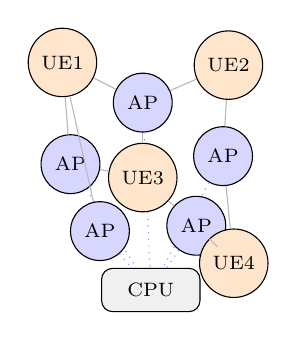
\begin{tikzpicture}[
                    scale=0.68,
                    ap/.style={draw, circle, fill=blue!16, minimum size=0.55cm, font=\scriptsize},
                    ue/.style={draw, circle, fill=orange!20, minimum size=0.55cm, font=\scriptsize},
                    cpu/.style={draw, rounded corners, fill=gray!12, minimum width=1.25cm, minimum height=0.55cm, font=\scriptsize},
                    link/.style={thin, gray!55},
                    front/.style={thin, blue!45, dotted}
                ]
                \node[cpu] (cpu) at (1.5,-2.35) {CPU};
                \foreach \x/\y/\i in {0/0/1, 1.35/1.15/2, 2.85/0.15/3, 0.55/-1.25/4, 2.35/-1.15/5}{
                        \node[ap] (ap\i) at (\x,\y) {AP};
                        \draw[front] (ap\i) -- (cpu);
                    }
                \node[ue] (u1) at (-0.15,1.9) {UE1};
                \node[ue] (u2) at (2.95,1.85) {UE2};
                \node[ue] (u3) at (1.35,-0.25) {UE3};
                \node[ue] (u4) at (3.05,-1.85) {UE4};

                \foreach \u/\a in {u1/ap1,u1/ap2,u1/ap4,u2/ap2,u2/ap3,u3/ap1,u3/ap2,u3/ap5,u4/ap3,u4/ap5}{
                        \draw[link] (\u) -- (\a);
                    }
            \end{tikzpicture}
        \end{column}
    \end{columns}
\end{frame}

\begin{frame}{System Model: Channels and Coherence Block}
    \small
    \begin{columns}[T,onlytextwidth]
        \begin{column}{0.50\textwidth}
            \textbf{Channel between AP $l$ and UE $k$}
            \[
                \mathbf{h}_{lk} = \sqrt{\beta_{lk}}\,\mathbf{g}_{lk},
                \qquad
                \mathbf{g}_{lk}\sim\mathcal{CN}(\mathbf{0},\mathbf{I}_N)
            \]
            \begin{tightitemize}
                \item $L$ APs, $K$ UEs, $N$ antennas per AP.
                \item $\beta_{lk}$ captures pathloss and shadowing.
                \item Dominant APs/beams are the useful structure for pilot assignment.
            \end{tightitemize}

            \vspace{0.55em}
            \textbf{Spectral efficiency form}
            \[
                \se_k =
                \left(1-\frac{\taup}{\tauc}\right)
                \log_2(1+\mathrm{SINR}_k)
            \]
        \end{column}
        \begin{column}{0.46\textwidth}
            \textbf{Coherence block}
            \vspace{0.4em}
            \begin{center}
                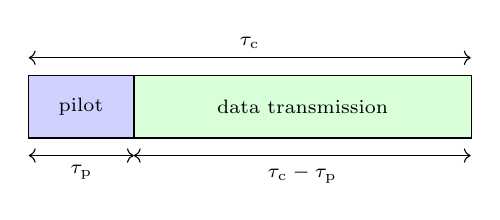
\begin{tikzpicture}[
                    scale=0.92,
                    every node/.style={font=\scriptsize}
                ]
                    \draw[thick] (0,0) rectangle (6.1,0.85);
                    \fill[blue!18] (0,0) rectangle (1.45,0.85);
                    \fill[green!15] (1.45,0) rectangle (6.1,0.85);
                    \draw[thick] (1.45,0) -- (1.45,0.85);
                    \node at (0.72,0.43) {pilot};
                    \node at (3.78,0.43) {data transmission};
                    \draw[<->,thin] (0,-0.25) -- node[below] {$\taup$} (1.45,-0.25);
                    \draw[<->,thin] (1.45,-0.25) -- node[below] {$\tauc-\taup$} (6.1,-0.25);
                    \draw[<->,thin] (0,1.10) -- node[above] {$\tauc$} (6.1,1.10);
                \end{tikzpicture}
            \end{center}

            \vspace{0.6em}
            \begin{block}{Key tension}
                More pilot symbols can reduce reuse pressure, but they leave fewer symbols for data.
            \end{block}
        \end{column}
    \end{columns}
\end{frame}

\begin{frame}{Uplink Pilots and Channel Estimation}
    \footnotesize
    \begin{columns}[T,onlytextwidth]
        \begin{column}{0.56\textwidth}
            \textbf{Pilot observation at AP $l$}
            \begin{align*}
                \mathbf{Y}_{l}^{p}
                &= \sum_{i=1}^{K}\sqrt{p_i}\,\mathbf{h}_{li}\boldsymbol{\phi}_{t_i}^{T}
                   + \mathbf{N}_{l},\\
                \mathbf{y}_{lk}^{p}
                &= \mathbf{Y}_{l}^{p}\boldsymbol{\phi}_{t_k}^{*}\\
                &= \sqrt{p_k}\taup\mathbf{h}_{lk}
                   + \sum_{i\in\mathcal{P}_k\setminus\{k\}}
                   \sqrt{p_i}\taup\mathbf{h}_{li}
                   + \mathbf{n}_{lk}.
            \end{align*}
            \[
                \mathcal{P}_k=\{i: t_i=t_k\}
            \]
        \end{column}
        \begin{column}{0.40\textwidth}
            \textbf{Interpretation}
            \begin{tightitemize}
                \item UE $k$ transmits pilot $\boldsymbol{\phi}_{t_k}$.
                \item AP $l$ correlates the received signal with that pilot.
                \item If another UE uses the same pilot, its channel enters the same statistic.
                \item The estimate is then contaminated before data detection starts.
            \end{tightitemize}

            \vspace{0.7em}
            \begin{block}{Pilot contamination}
                Same pilot plus overlapping strong channels creates mixed channel estimates.
            \end{block}
        \end{column}
    \end{columns}
\end{frame}

\begin{frame}{Pilot Contamination from Many-to-Many Serving}
    \footnotesize
    \begin{columns}[T,onlytextwidth]
        \begin{column}{0.48\textwidth}
            \textbf{Why assignment is difficult}
            \begin{tightitemize}
                \item Orthogonal pilot count is limited: usually $\taup<K$.
                \item Pilot reuse is therefore necessary.
                \item Each UE can overlap with many other UEs across APs and beams.
                \item A high-overlap same-pilot pair lowers channel-estimation quality and SINR.
            \end{tightitemize}

            \vspace{0.35em}
            \textbf{Graph view}
            \begin{tightitemize}
                \item Node = UE.
                \item Edge = strong effective conflict.
                \item Color = pilot index.
            \end{tightitemize}

            \vspace{0.2em}
            \begin{block}{Research question}
                Which UEs can reuse a pilot without creating a strong effective conflict?
            \end{block}
        \end{column}
        \begin{column}{0.48\textwidth}
            \centering
            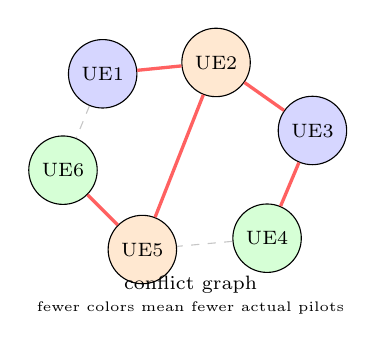
\begin{tikzpicture}[
                scale=0.72,
                ueA/.style={draw, circle, fill=blue!16, minimum size=0.62cm, font=\scriptsize},
                ueB/.style={draw, circle, fill=orange!18, minimum size=0.62cm, font=\scriptsize},
                ueC/.style={draw, circle, fill=green!16, minimum size=0.62cm, font=\scriptsize},
                edge/.style={very thick, red!62},
                weak/.style={thin, gray!45, dashed},
                every node/.style={font=\scriptsize}
            ]
                \node[ueA] (u1) at (0,1.7) {UE1};
                \node[ueB] (u2) at (2.0,1.9) {UE2};
                \node[ueA] (u3) at (3.7,0.7) {UE3};
                \node[ueC] (u4) at (2.9,-1.2) {UE4};
                \node[ueB] (u5) at (0.7,-1.4) {UE5};
                \node[ueC] (u6) at (-0.7,0.0) {UE6};

                \draw[edge] (u1) -- (u2);
                \draw[edge] (u2) -- (u3);
                \draw[edge] (u2) -- (u5);
                \draw[edge] (u3) -- (u4);
                \draw[edge] (u5) -- (u6);
                \draw[weak] (u1) -- (u6);
                \draw[weak] (u4) -- (u5);

                \node[align=center] at (1.55,-2.20) {conflict graph\\{\tiny fewer colors mean fewer actual pilots}};
            \end{tikzpicture}
        \end{column}
    \end{columns}
\end{frame}

% ----------------------------------------------------------------
% 3. Tradeoff
% ----------------------------------------------------------------
\section{Motivation}

\begin{frame}{Design Tradeoff: Contamination vs Overhead}
    \small
    \begin{center}
        \large
        \[
            \se_k =
            \left(1 - \frac{\taup}{\tauc}\right)
            \log_2\!\left(1+\mathrm{SINR}_k\right)
        \]
    \end{center}

    \vspace{0.4em}
    \begin{columns}[T,onlytextwidth]
        \begin{column}{0.48\textwidth}
            \textbf{More pilots}
            \begin{tightitemize}
                \item More orthogonal pilot resources.
                \item Lower pilot reuse pressure.
                \item Higher training overhead.
                \item Less data time in the coherence block.
            \end{tightitemize}
        \end{column}
        \begin{column}{0.48\textwidth}
            \textbf{Fewer pilots}
            \begin{tightitemize}
                \item Larger prelog factor.
                \item Better data-time efficiency.
                \item Higher contamination risk.
                \item Works only if the retained structure keeps SINR strong.
            \end{tightitemize}
        \end{column}
    \end{columns}

    \vspace{0.8em}
    \begin{block}{Main lens}
        A useful assignment should reduce pilot overhead without throwing away too much channel quality.
    \end{block}
\end{frame}

% ----------------------------------------------------------------
% 4. Starting papers
% ----------------------------------------------------------------
\begin{frame}{Starting Point: Gao and Mussbah}
    \small
    \begin{columns}[T,onlytextwidth]
        \begin{column}{0.48\textwidth}
            \textbf{Gao et al.}
            \begin{tightitemize}
                \item AP-domain pilot assignment.
                \item Many-to-many matching idea.
                \item Strong small-pilot regime result.
                \item Pilot count is a fixed design input.
            \end{tightitemize}
        \end{column}
        \begin{column}{0.48\textwidth}
            \textbf{Mussbah et al.}
            \begin{tightitemize}
                \item Beam-domain active/moderate beam graph.
                \item Conflict graph colored by DSATUR.
                \item Actual pilot count can become adaptive.
                \item RF-chain activity matters for EE.
            \end{tightitemize}
        \end{column}
    \end{columns}

    \vspace{0.9em}
    \centering
    \resizebox{0.92\linewidth}{!}{%
        \begin{tabular}{lccc}
            \toprule
            Family       & Domain                  & Conflict signal                & Pilot-count rule        \\
            \midrule
            Gao          & AP / large-scale fading & UE--AP matching                & fixed design budget     \\
            Mussbah      & beam domain             & active/moderate beam overlap   & graph chromatic number  \\
            Proposed set & AP + beam variants      & sparsified effective conflicts & adaptive where possible \\
            \bottomrule
        \end{tabular}
    }
\end{frame}

% ----------------------------------------------------------------
% 5. Reproduction anchor
% ----------------------------------------------------------------
\section{Reproduction}

\begin{frame}{Reproduction Anchor: Gao Small-Pilot Regime}
    \small
    \begin{columns}[T,onlytextwidth]
        \begin{column}{0.40\textwidth}
            \textbf{What this slide supports}
            \begin{tightitemize}
                \item 200 Monte Carlo setups.
                \item $\taup=10$, max-min power.
                \item Gao vs Random: \textbf{+21.7\%}.
                \item Paper claim: approximately +23\%.
            \end{tightitemize}

            \vspace{0.6em}
            \textbf{How to use it}
            \begin{tightitemize}
                \item Use as a reproduction anchor.
                \item Do not use it as the final multi-antenna benchmark.
            \end{tightitemize}

            \envnote{Environment: Gao reproduction setting; different from the common-ground multi-antenna results.}
        \end{column}
        \begin{column}{0.56\textwidth}
            \centering
            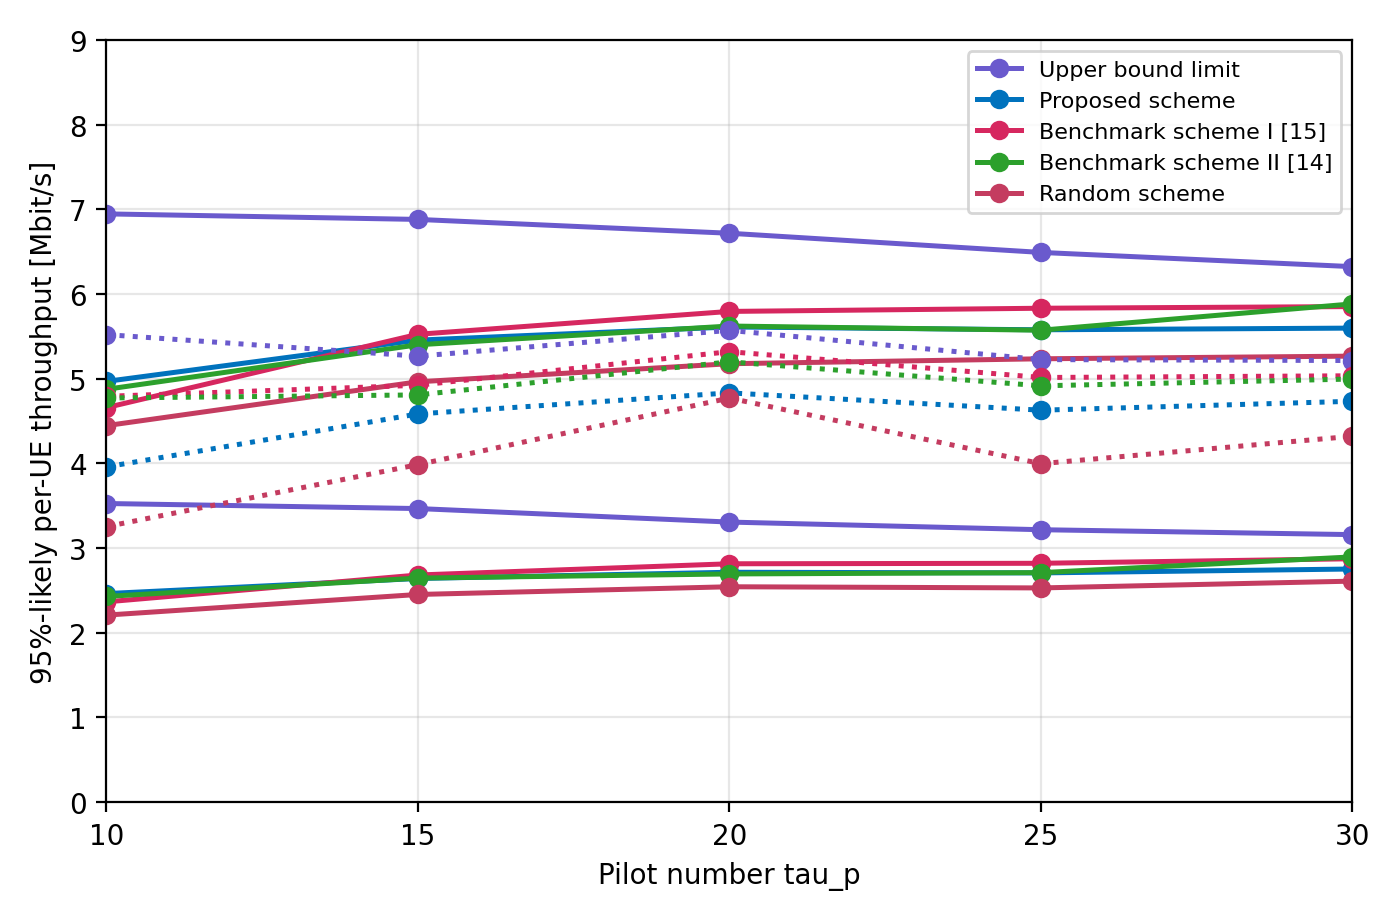
\includegraphics[width=\linewidth,height=0.63\textheight,keepaspectratio]{gao_fig3_vs_pilot_number_final200.png}
        \end{column}
    \end{columns}
\end{frame}

% ----------------------------------------------------------------
% 6. Proposed methods
% ----------------------------------------------------------------
\section{Method Family}

\begin{frame}{Proposed Method Family}
    \small
    \begin{columns}[T,onlytextwidth]
        \begin{column}{0.31\textwidth}
            \textbf{AP-Top8 Adaptive}
            \begin{tightitemize}
                \item Strongest 8 APs per UE.
                \item Conflict by shared Top-8 APs.
                \item Adaptive graph coloring.
            \end{tightitemize}

            \vspace{0.45em}
            \centering
            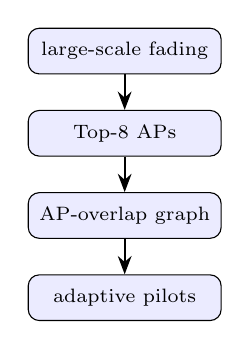
\begin{tikzpicture}[node distance=0.45cm,
                    box/.style={draw, rounded corners, fill=blue!8, align=center, font=\scriptsize,
                            minimum width=2.45cm, minimum height=0.58cm},
                    arr/.style={->, thick, >=Stealth}]
                \node[box] (a) {large-scale fading};
                \node[box, below=of a] (b) {Top-8 APs};
                \node[box, below=of b] (c) {AP-overlap graph};
                \node[box, below=of c] (d) {adaptive pilots};
                \draw[arr] (a) -- (b);
                \draw[arr] (b) -- (c);
                \draw[arr] (c) -- (d);
            \end{tikzpicture}
        \end{column}

        \begin{column}{0.31\textwidth}
            \textbf{Beam-Weighted Threshold}
            \begin{tightitemize}
                \item Active/moderate beam split.
                \item Higher weight for active-active overlap.
                \item Threshold weak conflicts.
            \end{tightitemize}

            \vspace{0.45em}
            \centering
            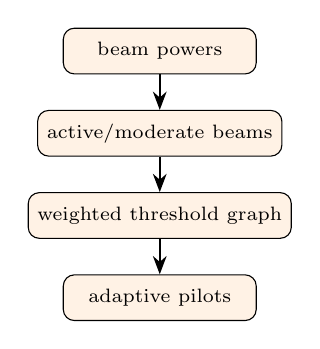
\begin{tikzpicture}[node distance=0.45cm,
                box/.style={draw, rounded corners, fill=orange!10, align=center, font=\scriptsize,
                    minimum width=2.45cm, minimum height=0.58cm},
                arr/.style={->, thick, >=Stealth}]
                \node[box] (a) {beam powers};
                \node[box, below=of a] (b) {active/moderate beams};
                \node[box, below=of b] (c) {weighted threshold graph};
                \node[box, below=of c] (d) {adaptive pilots};
                \draw[arr] (a) -- (b);
                \draw[arr] (b) -- (c);
                \draw[arr] (c) -- (d);
            \end{tikzpicture}
        \end{column}

        \begin{column}{0.31\textwidth}
            \textbf{Beam-Resource Matching}
            \begin{tightitemize}
                \item Candidate AP-beam resources.
                \item Many-to-many UE-resource matching.
                \item Adaptive pilot grouping.
            \end{tightitemize}

            \vspace{0.45em}
            \centering
            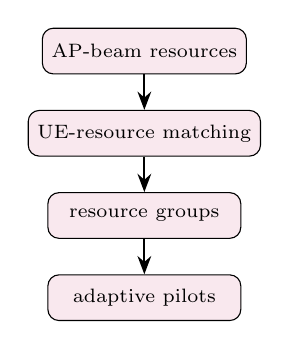
\begin{tikzpicture}[node distance=0.45cm,
                box/.style={draw, rounded corners, fill=purple!9, align=center, font=\scriptsize,
                    minimum width=2.45cm, minimum height=0.58cm},
                arr/.style={->, thick, >=Stealth}]
                \node[box] (a) {AP-beam resources};
                \node[box, below=of a] (b) {UE-resource matching};
                \node[box, below=of b] (c) {resource groups};
                \node[box, below=of c] (d) {adaptive pilots};
                \draw[arr] (a) -- (b);
                \draw[arr] (b) -- (c);
                \draw[arr] (c) -- (d);
            \end{tikzpicture}
        \end{column}
    \end{columns}
\end{frame}

% ----------------------------------------------------------------
% 7. Algorithm map
% ----------------------------------------------------------------
\begin{frame}{Method Map}
    \small
    \centering
    \resizebox{\linewidth}{!}{%
        \begin{tabular}{lcccc}
            \toprule
            Method                  & Domain & Conflict signal           & Pilot count & Role       \\
            \midrule
            Random                  & AP     & none                      & fixed       & reference  \\
            Gao Matching            & AP     & UE--AP matching           & fixed       & reference  \\
            Mussbah Beam Graph      & beam   & binary beam overlap       & adaptive    & reference  \\
            AP-Top8 Adaptive        & AP     & Top-8 AP overlap          & adaptive    & proposed   \\
            Beam-Weighted Threshold & beam   & weighted beam overlap     & adaptive    & proposed   \\
            Beam-Resource Matching  & beam   & AP-beam resource matching & adaptive    & proposed   \\
            \bottomrule
        \end{tabular}
    }

    \vspace{1.0em}
    \begin{block}{Unifying view}
        Different conflict signals, same lever: reduce effective conflicts while keeping dominant channel structure.
    \end{block}
\end{frame}

% ----------------------------------------------------------------
% 8. Main result
% ----------------------------------------------------------------
\section{Results}

\begin{frame}{Main Result: User-Load Crossover in SE}
    \small
    \centering
    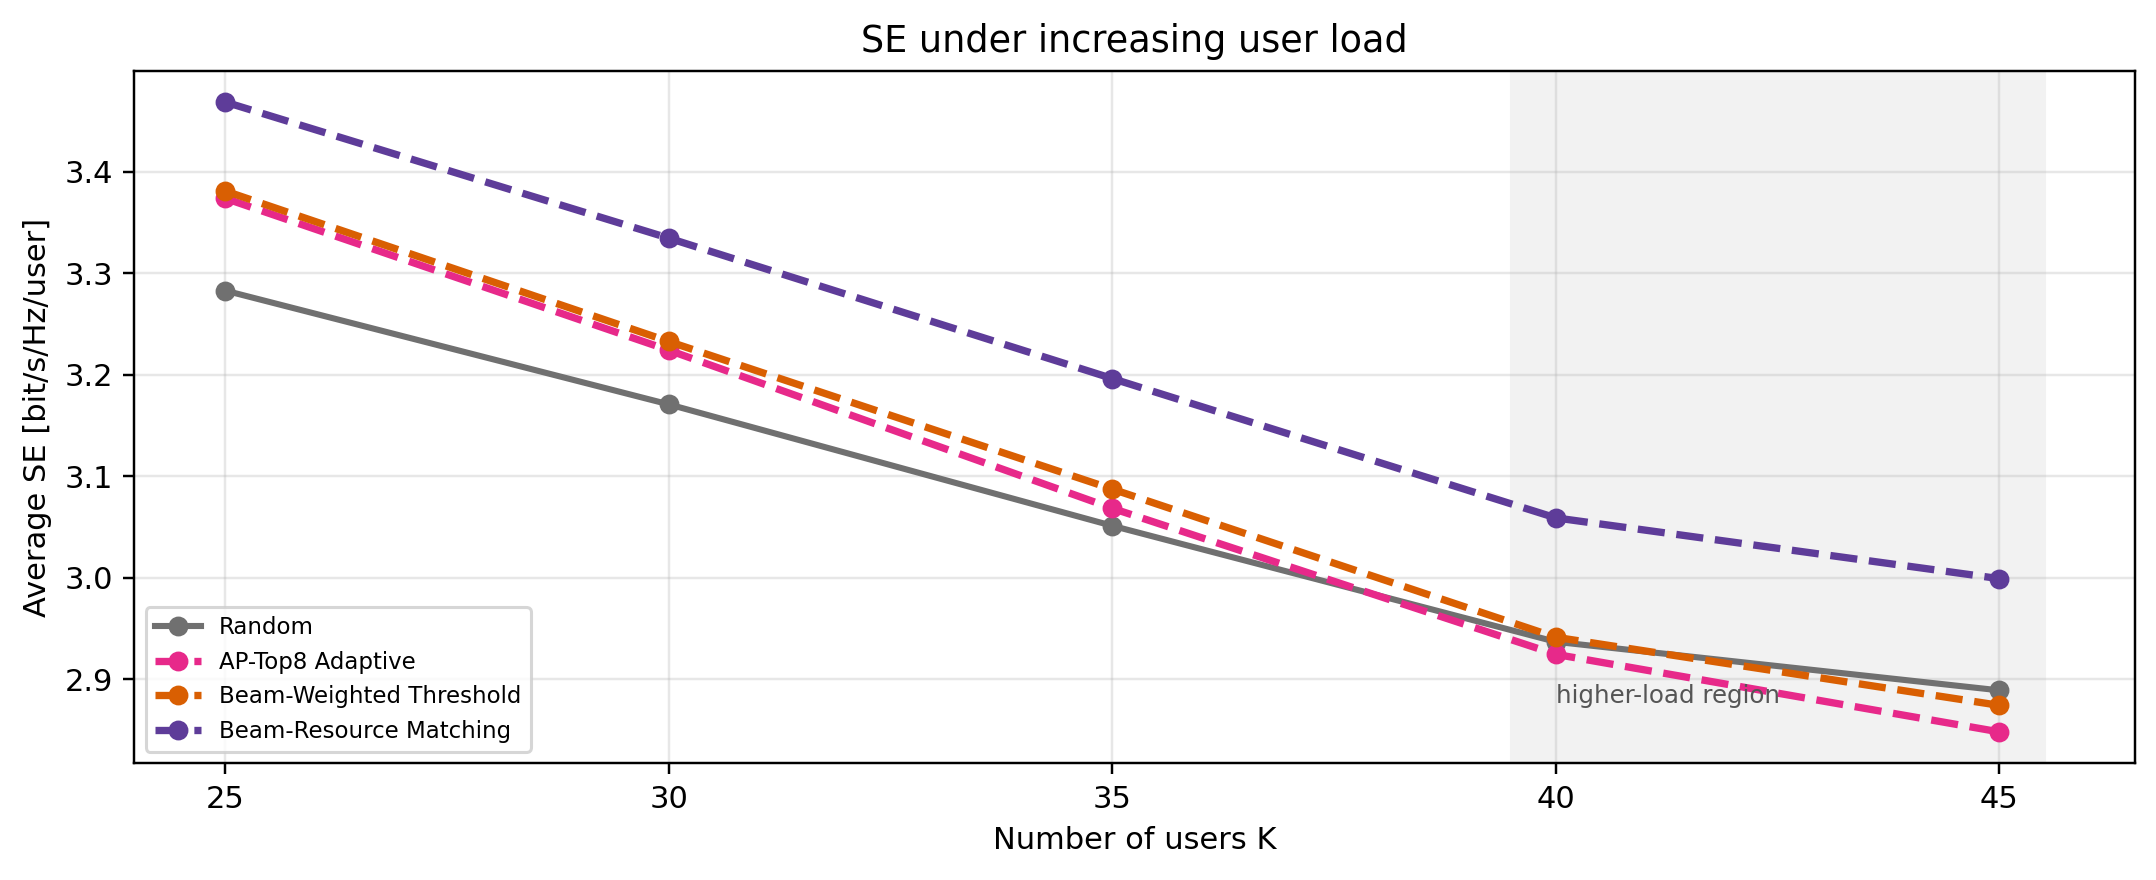
\includegraphics[width=0.90\linewidth,height=0.56\textheight,keepaspectratio]{presentation_clean_k_sweep_se.png}

    \vspace{0.15em}
    \begin{columns}[T,onlytextwidth]
        \begin{column}{0.47\textwidth}
            \scriptsize
            \textbf{Environment:} $K=25,\ldots,45$, $L=100$, $N=8$, $\tauc=100$, $\taup^{design}=10$, 200 setups, closed-form SE.
        \end{column}
        \begin{column}{0.49\textwidth}
            \scriptsize
            \textbf{Reading:} AP-Top8 and Beam-Weighted cross below Random at high load; Beam-Resource Matching remains positive at $K=45$ (\textbf{+3.81\%}).
        \end{column}
    \end{columns}
\end{frame}

% ----------------------------------------------------------------
% 9. Mechanism
% ----------------------------------------------------------------
\begin{frame}{Mechanism: Pilot Count vs SINR Balance}
    \small
    \begin{columns}[T,onlytextwidth]
        \begin{column}{0.44\textwidth}
            \textbf{Common-ground snapshot}
            \begin{center}
                \scriptsize
                \resizebox{\linewidth}{!}{%
                    \begin{tabular}{lccc}
                        \toprule
                        Method                  & $\bar{\tau}_{p}$ & prelog ratio & SE gain  \\
                        \midrule
                        Random                  & 14.94            & baseline     & baseline \\
                        Beam-Weighted Threshold & 3.23             & +8.67\%      & +8.53\%  \\
                        Beam-Resource Matching  & 4.46             & +7.76\%      & +7.80\%  \\
                        AP-Top8 Adaptive        & 7.90             & +5.21\%      & +5.28\%  \\
                        \bottomrule
                    \end{tabular}
                }
            \end{center}

            \vspace{0.5em}
            \textbf{Reading}
            \begin{tightitemize}
                \item Fewer pilots improve the prelog factor.
                \item Too much pruning can damage SINR under high load.
                \item The useful target is balance, not the minimum possible pilot count.
            \end{tightitemize}
        \end{column}
        \begin{column}{0.52\textwidth}
            \centering
            
\includegraphics[width=\linewidth,height=0.64\textheight,keepaspectratio]{presentation_clean_pilot_box.png}
        \end{column}
    \end{columns}
\end{frame}

% ----------------------------------------------------------------
% 10. Energy efficiency
% ----------------------------------------------------------------
\begin{frame}{Energy Efficiency Under User Load}
    \small
    \centering
    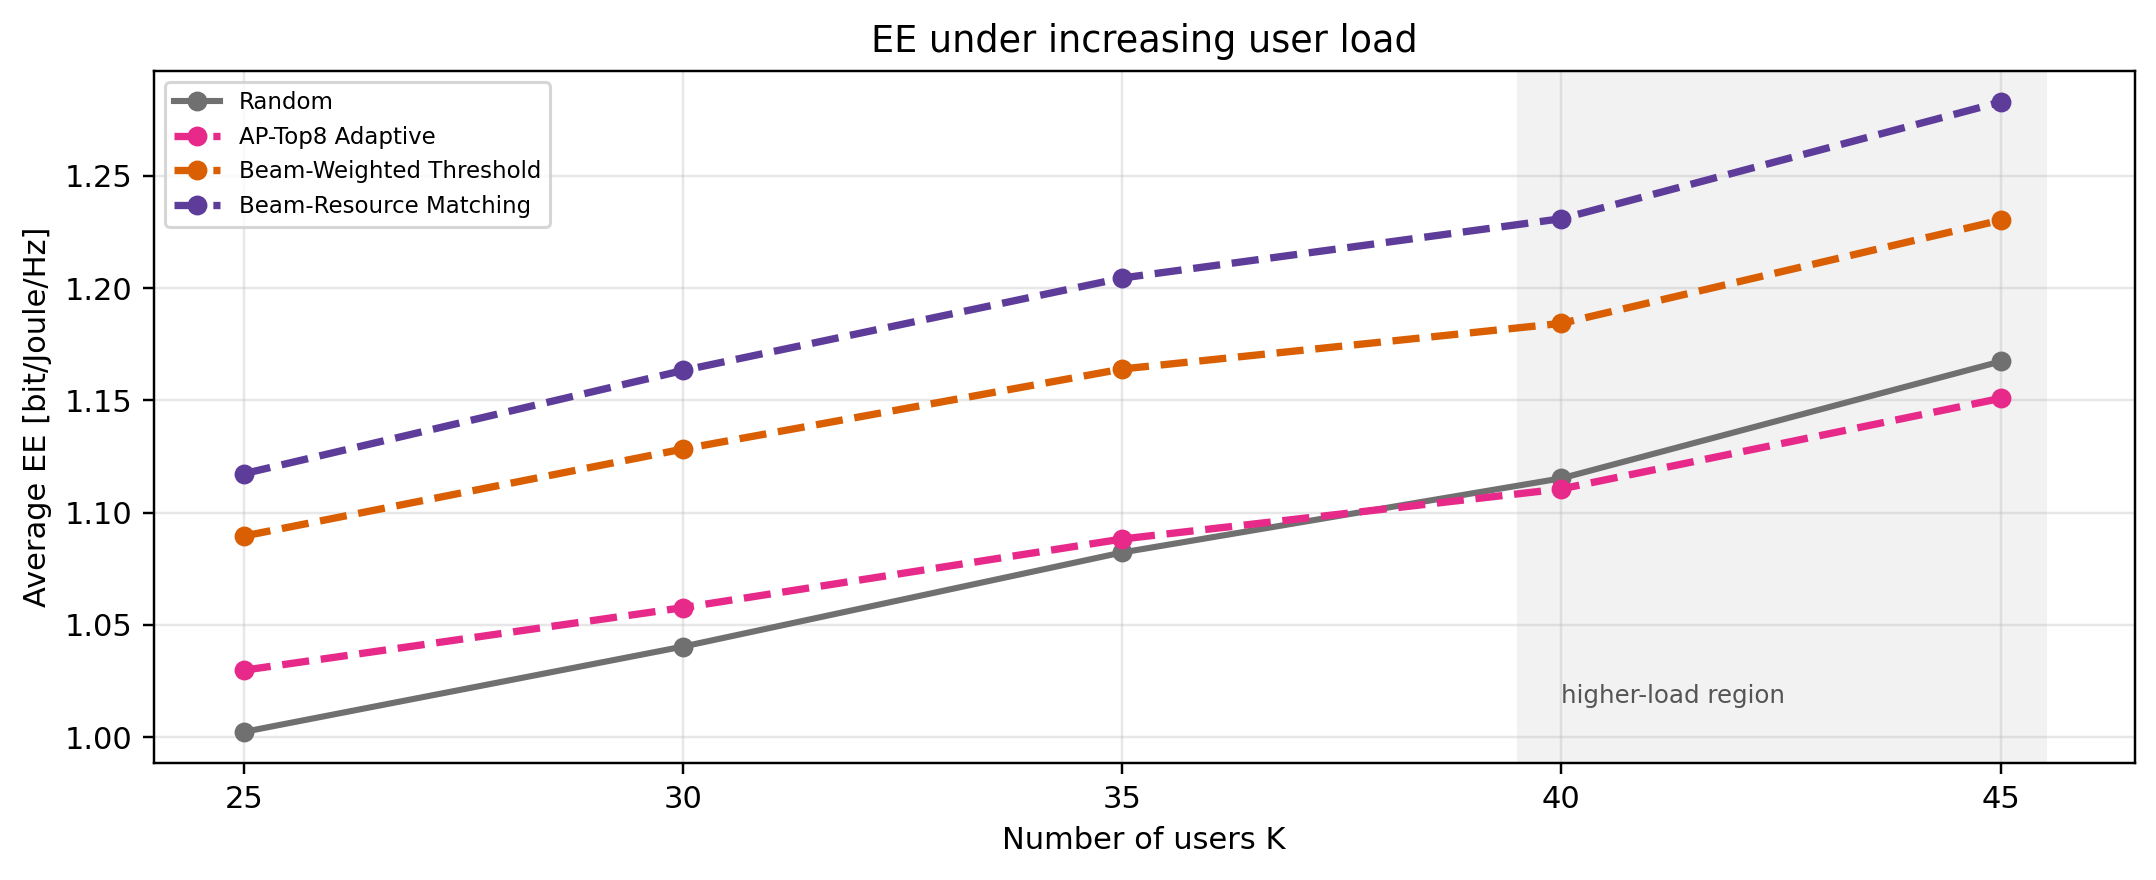
\includegraphics[width=0.90\linewidth,height=0.56\textheight,keepaspectratio]{presentation_clean_k_sweep_ee.png}

    \vspace{0.15em}
    \begin{columns}[T,onlytextwidth]
        \begin{column}{0.47\textwidth}
            \scriptsize
            \textbf{Environment:} $L=100$, $N=8$, $\tauc=100$, $\taup^{design}=10$, 200 setups, closed-form SE/EE proxy.
        \end{column}
        \begin{column}{0.49\textwidth}
            \scriptsize
            \textbf{At $K=45$ vs Random:} Beam-Resource \textbf{+9.90\%}, Beam-Weighted \textbf{+5.39\%}, AP-Top8 \textbf{-1.41\%}.
        \end{column}
    \end{columns}
\end{frame}

% ----------------------------------------------------------------
% 11. Conclusion
% ----------------------------------------------------------------
\section{Conclusion}

\begin{frame}{Conclusion}
    \small
    \begin{center}
        \large
        \textbf{Pilot assignment is a balance problem.}\\
        \vspace{0.15em}
        \textbf{Prune enough to reduce pilots, but not enough to destroy SINR.}
    \end{center}

    \vspace{0.45em}
    \begin{columns}[T,onlytextwidth]
        \begin{column}{0.48\textwidth}
            \textbf{What we can defend}
            \begin{tightitemize}
                \item Gao gives a useful reproduction anchor.
                \item Multiple proposed methods sparsify conflicts.
                \item User-load crossover shows that pruning can overreach.
                \item Beam-Resource Matching is the most robust current direction.
            \end{tightitemize}
        \end{column}
        \begin{column}{0.48\textwidth}
            \textbf{What we should not oversell}
            \begin{tightitemize}
                \item Fewer pilots are not always better.
                \item $\taup=1$ is not the design conclusion.
                \item Cross-environment absolute SE should not be mixed.
                \item EE is a simplified proxy.
            \end{tightitemize}
        \end{column}
    \end{columns}

    \vspace{0.55em}
    \begin{center}
        \normalsize
        \textbf{Final claim:} good UE clustering and AP/beam pruning should balance SINR preservation against pilot-count reduction.
    \end{center}
\end{frame}

% ----------------------------------------------------------------
% Backup slides
% ----------------------------------------------------------------
\appendix
\section{Backup}

\begin{frame}{Backup: Closed-Form Environment And Load Sensitivity}
    \small
    \begin{columns}[T,onlytextwidth]
        \begin{column}{0.48\textwidth}
            \textbf{Separate closed-form environment}
            \begin{tightitemize}
                \item $K=30$, $L=100$, $N=8$.
                \item $\tauc=100$, $\taup^{design}=10$.
                \item 200 setups.
                \item Closed-form MMSE+MRC SE.
            \end{tightitemize}

            \vspace{0.45em}
            \begin{center}
                \scriptsize
                \begin{tabular}{lcc}
                    \toprule
                    Method                  & mean SE        & $\bar{\tau}_p$ \\
                    \midrule
                    Random                  & 3.171          & 10.00          \\
                    AP-Top8 Adaptive        & 3.224          & 8.34           \\
                    Beam-Weighted Threshold & 3.233          & 7.42           \\
                    Beam-Resource Matching  & \textbf{3.335} & \textbf{4.59}  \\
                    \bottomrule
                \end{tabular}
            \end{center}
        \end{column}
        \begin{column}{0.48\textwidth}
            \textbf{Closed-form K-sweep}
            \begin{center}
                \scriptsize
                \begin{tabular}{rccc}
                    \toprule
                    K  & AP-Top8 & Weighted & Resource matching \\
                    \midrule
                    25 & +2.77\% & +2.99\%  & \textbf{+5.66\%} \\
                    30 & +1.68\% & +1.96\%  & \textbf{+5.18\%} \\
                    35 & +0.57\% & +1.19\%  & \textbf{+4.76\%} \\
                    40 & -0.42\% & +0.15\%  & \textbf{+4.16\%} \\
                    45 & -1.42\% & -0.51\%  & \textbf{+3.81\%} \\
                    \bottomrule
                \end{tabular}
            \end{center}

            \begin{tightitemize}
                \item AP-domain Top-N weakens as load grows.
                \item Beam-Resource Matching remains strongest in this sweep.
            \end{tightitemize}
        \end{column}
    \end{columns}
\end{frame}

\begin{frame}{Backup: Graph Consistency Rules}
    \small
    \begin{tightenumerate}
        \item Use common-ground MC figures for the main ranking.
        \item Use method names, not person-specific labels.
        \item Use only Random, Gao Matching, and Mussbah Beam Graph as main references.
        \item Use Gao reproduction only as a small-pilot reproduction anchor.
        \item Say ``EE proxy'' for the current EE plots.
        \item Do not claim a $\taup=7$ optimum from the current tau sweep.
        \item Add bootstrap CI for the final 12-scheme run before using significance language.
    \end{tightenumerate}
\end{frame}

\end{document}
